\newpage
\section*{三、结果与分析}


\subsection*{1. 截止电压平均值与重复性}

记截止电压大小为 $U_s$（即预习中的 $U_a$），由带符号的仪表示值取 $U_{s,j}=-U_{AK,j}=|U_{AK,j}|$。每个波长的三个截止电压分别取平均，采用重复测量的统计方法评定平均值的 A 类标准不确定度。

\begin{equation}
\overline U_{s,i}=\frac13\sum_{j=1}^3 U_{s,ij},\qquad u_A(\overline U_{s,i})=\sqrt{\frac{\sum_{j=1}^3(U_{s,ij}-\overline U_{s,i})^2}{3(3-1)}}.
\end{equation}

频率按 $\nu=c/\lambda$ 计算，其中 $c=299792458\,\mathrm{m\,s^{-1}}$，波长先由nm换为m。下表保留中间计算位数。

\begin{center}\small\setstretch{1.0}
\renewcommand{\arraystretch}{1.25}
\begin{tabular}{|c|c|c|c|}
\hline
$\lambda$/nm & $\nu/(10^{14}\,\mathrm{Hz})$ & $\overline U_s$/V & $u_A(\overline U_s)$/V\\\hline
365 & 8.213492 & 1.372333 & 0.001453\\\hline
405 & 7.402283 & 0.988000 & 0.001528\\\hline
436 & 6.875974 & 0.790333 & 0.001202\\\hline
546 & 5.490704 & 0.252000 & 0.001732\\\hline
577 & 5.195710 & 0.118333 & 0.001453\\\hline
\end{tabular}
\end{center}


\subsection*{2. 截止电压—频率线性拟合}

令 $x=\nu/(10^{14}\,\mathrm{Hz})$，以五个平均截止电压作普通最小二乘拟合 $U_s=ax+b$。采用不加权拟合；误差仅表示各平均值的 A 类分量。

\begin{equation}
\frac{U_s}{\mathrm V}=0.40706790x-1.99695305,\qquad r=0.999170,\quad R^2=0.998340.
\end{equation}

\begin{figure}[H]\centering
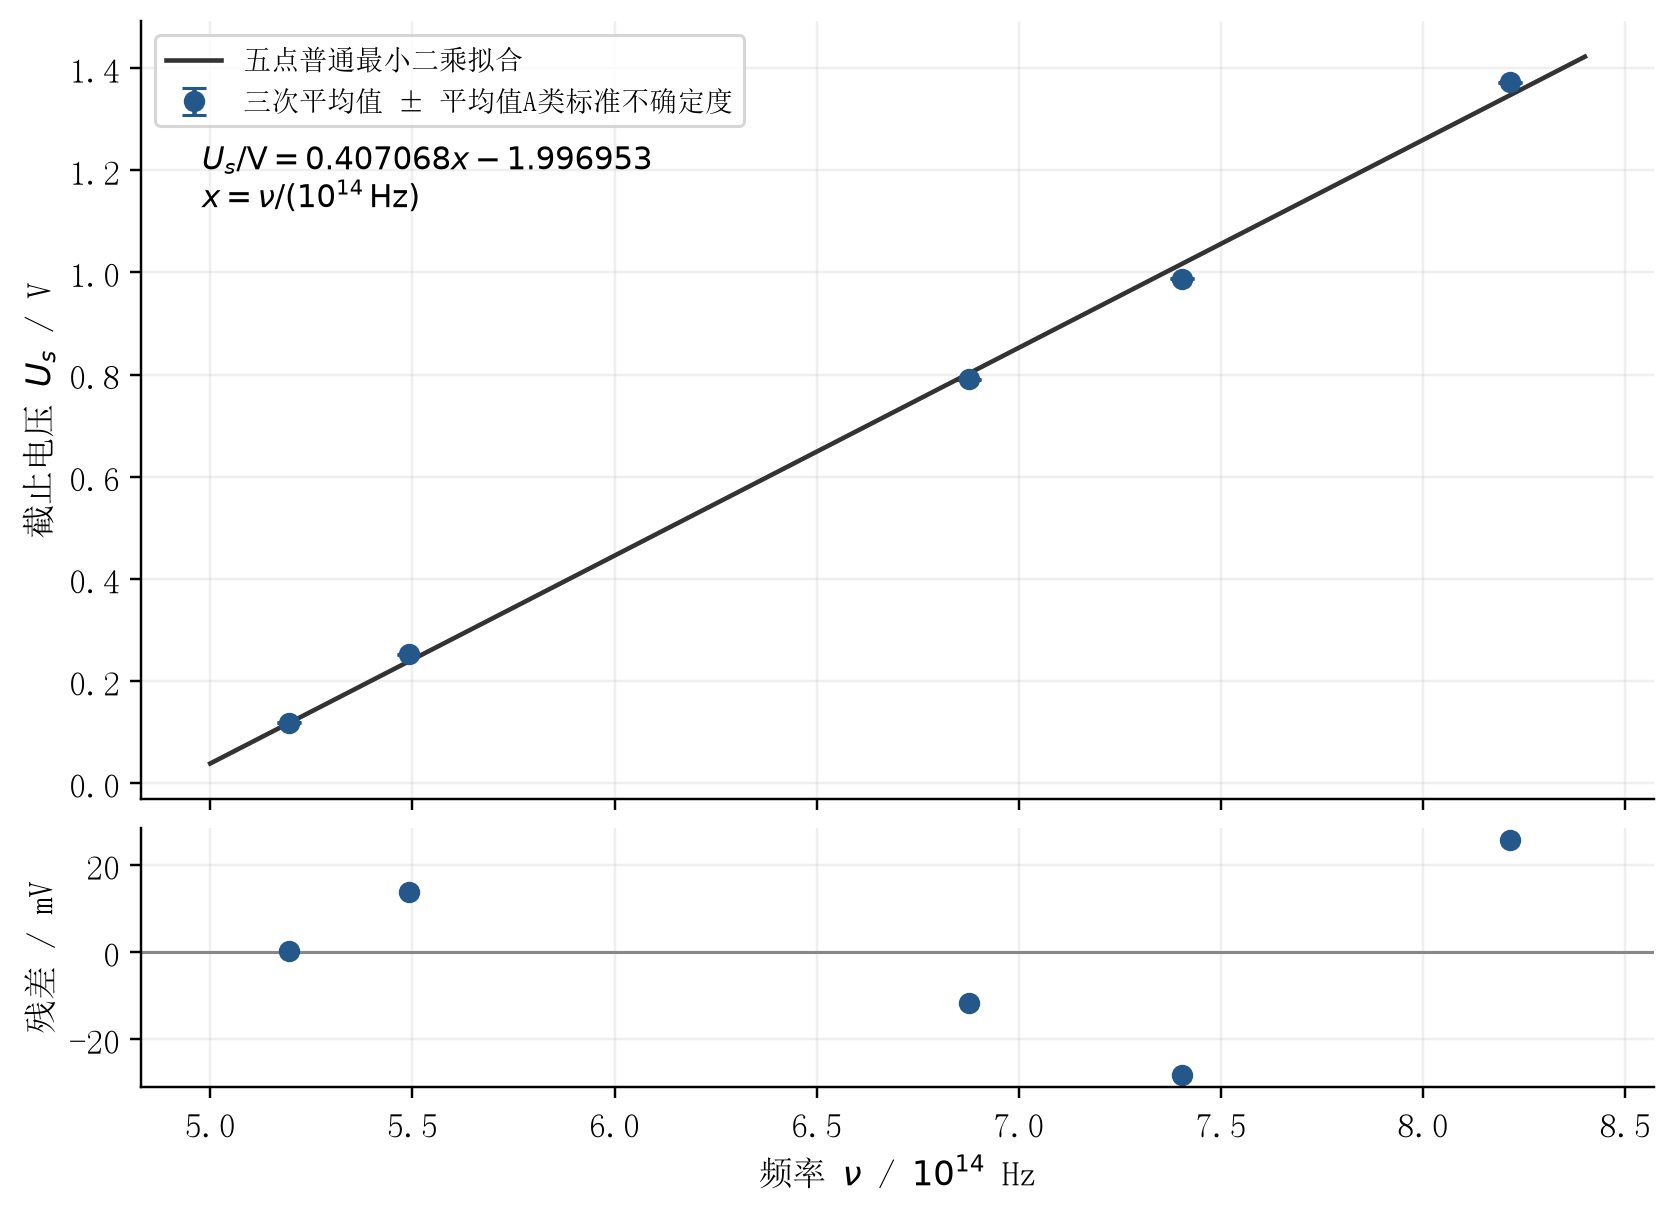
\includegraphics[height=7cm,width=0.98\linewidth,keepaspectratio]{../assets/cutoff_fit.png}
\caption{截止电压与频率的线性拟合及残差}
\end{figure}


\newpage
\subsection*{3. 普朗克常数及拟合标准不确定度}

由 $U_s=(h/e)\nu-W/e$，采用 $e=1.602176634\times10^{-19}\,\mathrm C$，有

\begin{equation}
k=a\times10^{-14}\,\mathrm s=4.0706790\times10^{-15}\,\mathrm{V\cdot s},\qquad h=ek.
\end{equation}

\begin{equation}
W=-eb,\qquad \nu_0=-\frac ba\times10^{14}\,\mathrm{Hz}.
\end{equation}

设 $S_{xx}=\sum(x_i-\bar x)^2$，残差为 $v_i=\overline U_{s,i}-(ax_i+b)$。拟合参数的标准误差与协方差为

\begin{equation}
s^2=\frac{\sum v_i^2}{5-2},\quad u^2(a)=\frac{s^2}{S_{xx}},\quad u^2(b)=s^2\left(\frac15+\frac{\bar x^2}{S_{xx}}\right),\quad C_{ab}=-\frac{\bar x s^2}{S_{xx}}.
\end{equation}

\noindent 本次残差平方和为 $0.00179647\,\mathrm{V^2}$。参数标准误差为 $u(a)=0.00958397\,\mathrm V$、$u(b)=0.06453045\,\mathrm V$，协方差为 $C_{ab}=-0.000609499\,\mathrm{V^2}$。斜率与截距相关，计算横轴截距的不确定度时保留协方差：

\begin{equation}
u(h)=e\,u(a)\times10^{-14}\,\mathrm s,\quad u(W)=e\,u(b),\quad u(\nu_0)=10^{14}\,\mathrm{Hz}\sqrt{\frac{u^2(b)}{a^2}+\frac{b^2u^2(a)}{a^4}-\frac{2bC_{ab}}{a^3}}.
\end{equation}

最终写为

\begin{equation}
\boxed{h=(6.52\pm0.15)\times10^{-34}\,\mathrm{J\cdot s}},
\end{equation}

\begin{equation}
\boxed{W=(2.00\pm0.06)\,\mathrm{eV}},\qquad \boxed{\nu_0=(4.91\pm0.05)\times10^{14}\,\mathrm{Hz}}.
\end{equation}

上述“$\pm$”均表示拟合标准不确定度，不是完整合成标准不确定度。


\subsection*{4. 与公认值比较}

以 $h_0=6.62607015\times10^{-34}\,\mathrm{J\cdot s}$ 为参考，使用未修约结果计算：

\begin{equation}
\frac{|h-h_0|}{h_0}\times100\%=1.57\%,\qquad \frac{u(h)}{|h|}\times100\%=2.35\%.
\end{equation}

前者为相对误差，后者为相对拟合标准不确定度。
重复测量的分散较小，而拟合残差可达约28 mV。这说明谱线间还存在零点偏移、滤光片带宽或零电流判定等影响导致误差。


\newpage
\subsection*{5. 伏安特性曲线}

\begin{figure}[H]\centering
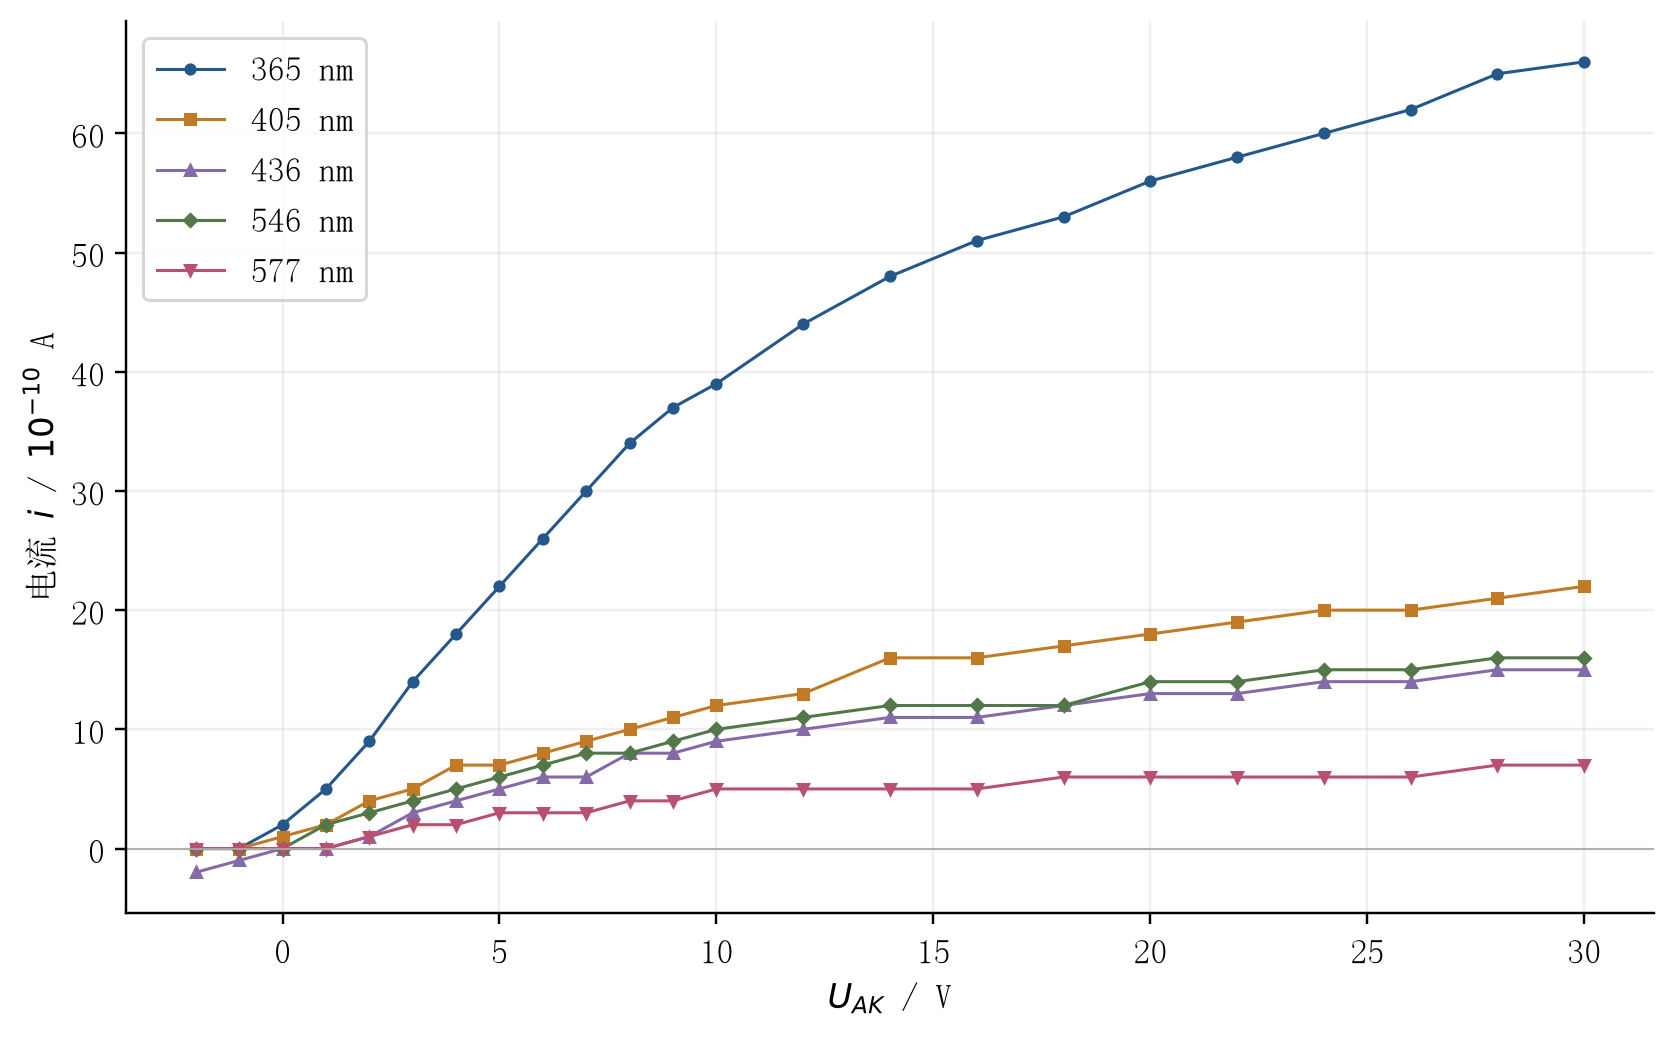
\includegraphics[height=9cm,width=0.98\linewidth,keepaspectratio]{../assets/iv_curves.png}
\caption{五种单色光的伏安特性；点间连线仅表示测量趋势}
\end{figure}

五条曲线的电流总体随阳极电压升高而增大，高电压段增速减缓，表现出趋于饱和的趋势。365 nm对应的电流最大，但不同滤光片透过率、汞灯各谱线强度及光电管响应均不同，所以不能据此断言“频率越高，饱和电流就一定越大”。
436 nm在 −2 V、−1 V处分别记录 $-2\times10^{-10}$ A、$-1\times10^{-10}$ A，明显大于零电压下记录的暗电流量级。它可能与阳极反向光电流、量程切换后的零点或现场读数状态有关。

\newpage
\subsection*{6. 光电流与光源距离、光阑孔径}

在波长及其他条件固定时，以 $i$ 对 $1/L^2$、$\Phi^2$ 作图。距离由mm换成m，孔径平方以 $\mathrm{mm^2}$ 表示。

\begin{figure}[H]\centering
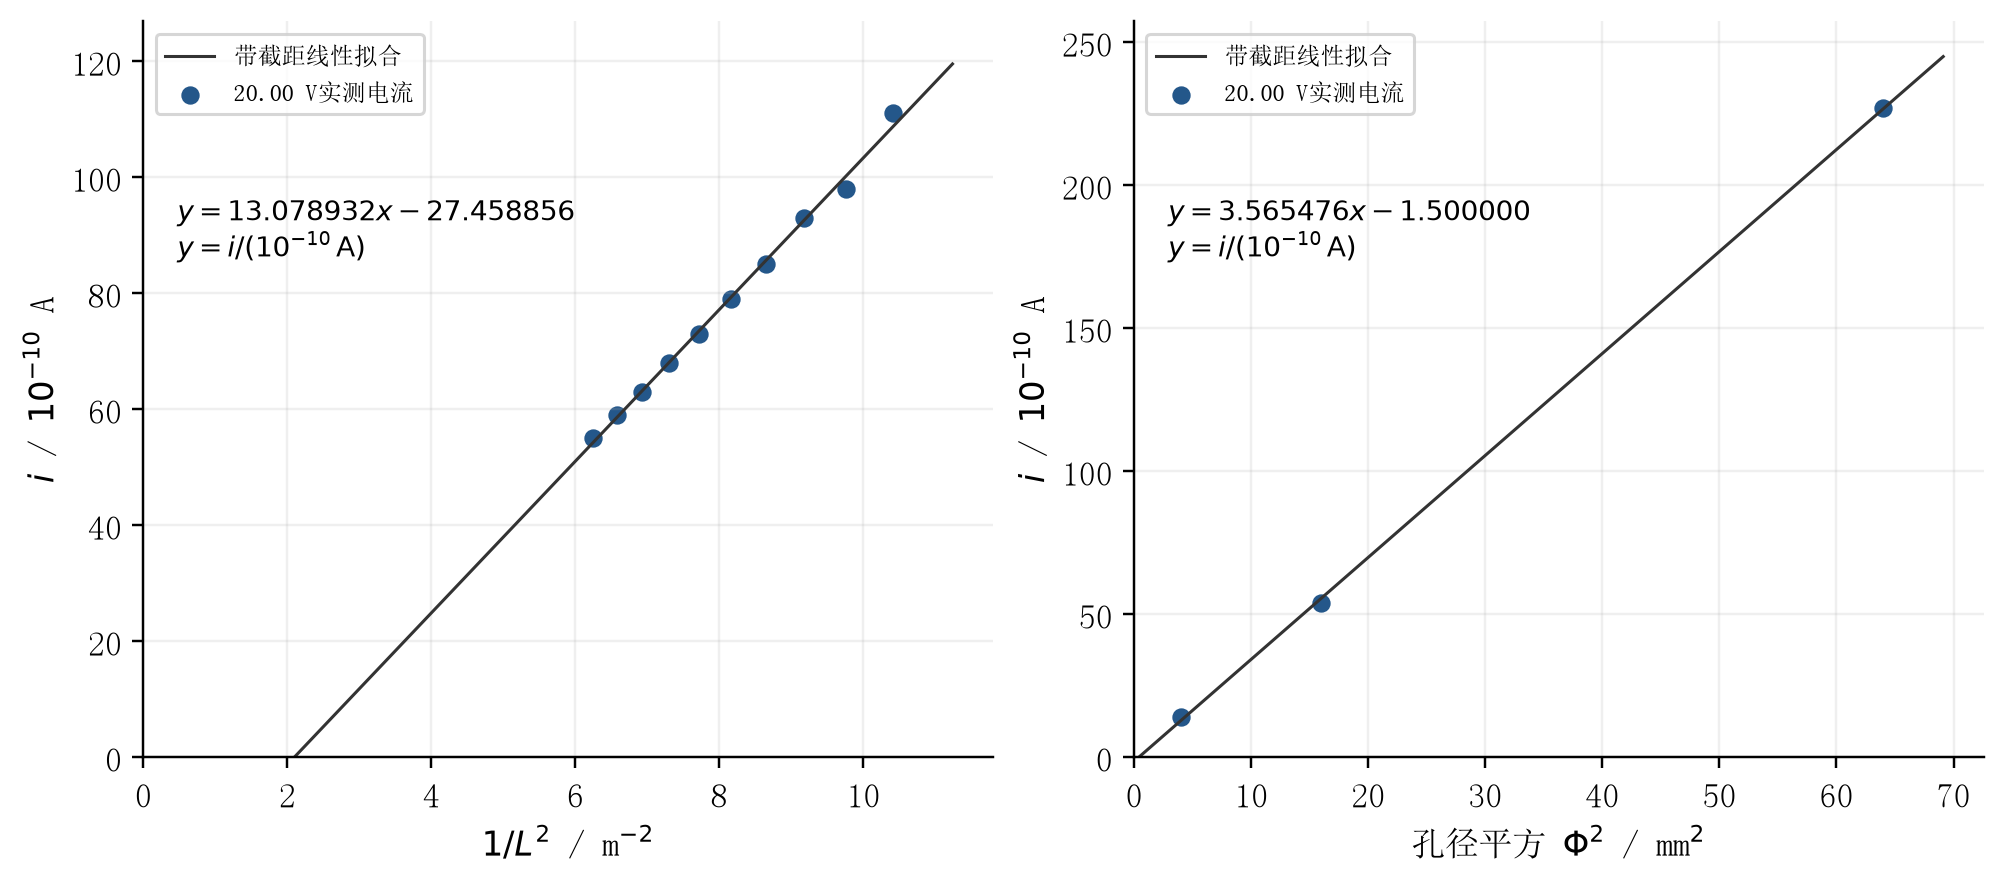
\includegraphics[height=7.1cm,width=0.98\linewidth,keepaspectratio]{../assets/intensity_relations.png}
\caption{20.00 V下的光电流与距离平方倒数、孔径平方的关系}
\end{figure}

\begin{equation}
\frac{i}{10^{-10}\,\mathrm A}=13.07893\frac{L^{-2}}{\mathrm{m^{-2}}}-27.45886,\qquad R^2=0.995884,
\end{equation}

\begin{equation}
\frac{i}{10^{-10}\,\mathrm A}=3.565476\frac{\Phi^2}{\mathrm{mm^2}}-1.500000,\qquad R^2=0.999843.
\end{equation}

距离缩短时电流增大，与入射光增强的趋势相符。但线性拟合截距明显偏离零，且 $iL^2$ 从400 mm处的8.80增加至310 mm处的10.6671（单位 $10^{-10}\,\mathrm{A\,m^2}$），增加约21.2\%。因此数据支持近似线性趋势，但不能严格验证其反平方正比的关系。
可能原因包括汞灯不是理想点光源、距离参考点偏差、光路接受范围以及20 V下未完全饱和。

孔径2、4、8 mm对应的面积比为 $1:4:16$，实测电流比为 $1:3.857:16.214$。与按2 mm读数归一化的比例值相比，后两点相差约3.57\%、1.34\%，较好地支持光电流随孔径面积增加。



\newpage
\subsection*{7. 误差分析}

\subsubsection*{（1）截止电压的零点判定}

本次用零电流法测量截止电压。电流未稳定或换档后未重新调零，都会影响过零位置，进而影响拟合斜率和普朗克常数。测量时应在零点附近缓慢细调，从一致方向接近零点，稳定后读数。

\subsubsection*{（2）暗电流与杂散光}

零电压下记录的暗电流为 $-3\times10^{-13}$ A，说明本底不完全为零。暗电流和漏入的杂散光会影响截止电压判定。应盖好遮光盖检查本底，并在测量时避免杂散光；本次仅记录一个暗电流值，不作电压修正。

\subsubsection*{（3）拓展实验未达到明显饱和}

365 nm光照下，电压从20 V增至30 V时，电流由 $56\times10^{-10}$ A增至 $66\times10^{-10}$ A，说明拓展实验所用的20 V尚未达到明显饱和。因此，距离和孔径实验只能比较该电压下的光电流，不能直接当作饱和电流分析。

\subsubsection*{（4）距离读数与光路对准}

距离实验中，$iL^2$ 随距离变化约21.2\%，偏离理想反平方关系，可能与距离参考点不一致、汞灯并非点光源有关。应统一距离起止位置；移动光电管或更换2、4、8 mm光阑时保持光路同轴，减少接收光量变化带来的误差。

